\chapter{Open Source Holography} % Main appendix title
\label{app:holog}

\section{Open-Source Holography}
\label{sec:appendix_hardware}

Figure~\ref{fig:setup} shows a schematic of the RF electronics.  Two local oscillators (LOs) produce signals between 10 and 13 GHz. The LO1 synthesizer produces a signal between 10 and 13\,GHz, while LO2 produces the same frequency with some offset $f_{\text{offset}}$ (this offset is chosen to be 10\,MHz).  The offset frequency is what will eventually produce an intermediate frequency exiting the mixer diplexers.  The purpose of the mixer diplexers is to ensure the signal from the first LO travels to the two mixers, and then ensures that the IF output of the mixers travels in the opposing direction down the RF chain to the FPGA.

The LO1 signal goes to the active multiplying chain, where it is multiplied by 8(12), obtaining frequencies in the F90(150)-band.  Prior to leaving the source horn, -10dB of the signal splits off, and mixes with LO2 in the harmonic mixer, producing an intermediate frequency IF$_1$ which then goes through one of the mixer diplexers and to the FPGA.  The rest of the signal leaves the source horn, through the components of the LATR optics, and the signal reaching the back of the optics tube mixes with LO2 in a GaAs harmonic mixer, and the subsequent intermediate frequency, IF$_2$, which also travels to the FPGA.  The FPGA used for these measurements is the Re-configurable Open Architecture Computing Hardware (ROACH-2) board, which correlates the reference and modulated signals~\cite{roach2}.

\begin{figure}[ht]
    \centering
    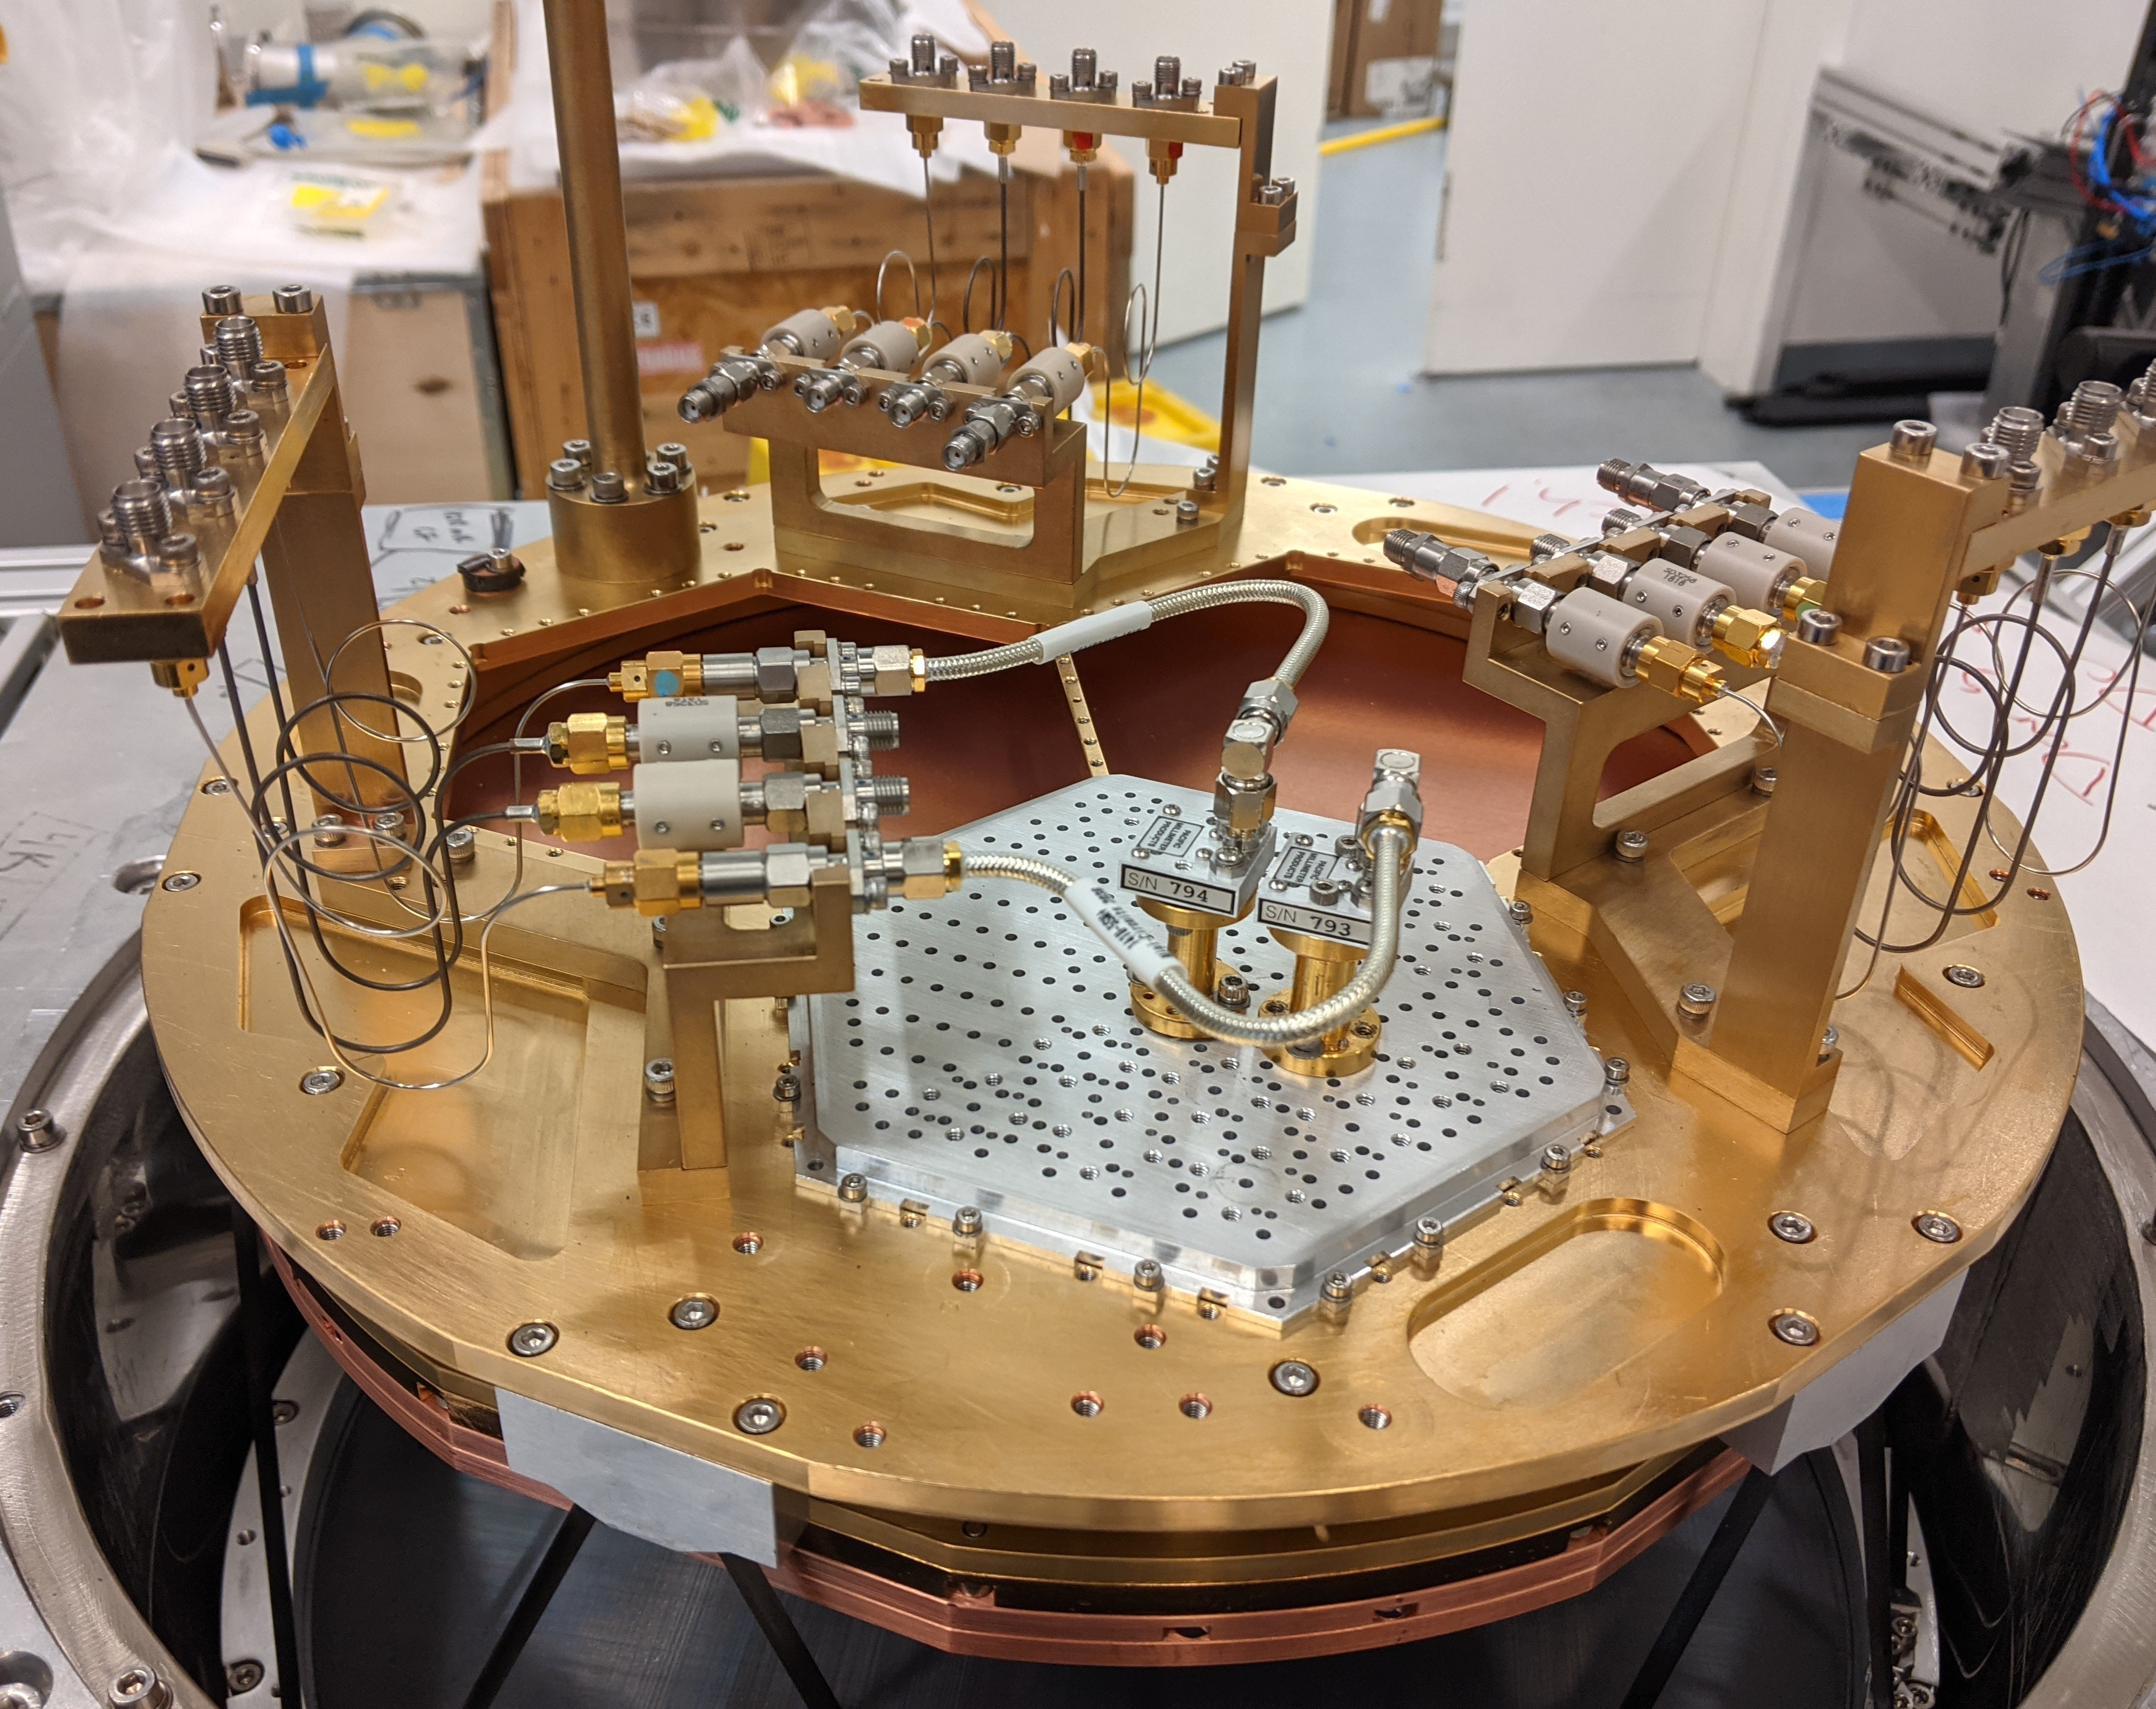
\includegraphics[width = .7\textwidth]{Figures/FPA.jpeg}
    \caption{The Simons Observatory Large Aperture Telescope optics tube focal plane readout, which is cooled to 4\,K during measurements.  The holography receivers (two receivers for redundancy) are approximately 7.4\,cm from the center of the focal plane.}
    \label{fig:fpa}
\end{figure}

The signal from the source(receiver) needs to be amplified due to high loss levels in the coax path from the harmonic mixer on the source to the reference mixer-diplexer (LATRt readout chain).  To overcome this loss, amplifiers with attenuators  increase the signal in the RF chain prior to entering the mixer diplexer.  The setup uses low phase variation coaxial cables leftover from the DASI experiment~\cite{CHURCH20031083}.  The phase repeatability of the holography setup is within $\approx3^{\circ}$.  We further note that any drift in the map would present itself in the phase map.  This phase drift would be removed during the propagation into the far-field when we optimize the position of the beam map in the LAT focal plane. 

The source moves in a 2-D grid above the LATRt with motorized XY stages~\cite{stages}.  The source mounts to the stages such that the signal points downwards towards the LATRt window.  The laboratory is over 7.5\,m tall, and therefore we expect reflection from the walls to be diffuse.  Therefore, the reflected signal is diluted before reflecting into the testing system.  The dominant reflections are from reflections within the optics tube, as the hexagon side-lobe is the dominant side-lobe feature in the beam maps (Figure~\ref{fig:beam_measurements_all}).
Figure~\ref{fig:fpa} shows the holography receiver readout at the back of the optics tube focal plane.  An SO MF feedhorn array is adapted for the holography experiment.  On the readout side of the array, attachment screws are added for attaching a circular to rectangular transition waveguide.  The transition waveguide connects the back of the focal plane (circular) to the GaAs W-band harmonic mixer (rectangular).  Though the design of the W-band harmonic mixer is optimized for F90 frequency readout, the W-band harmonic mixer is used for both F90 and F150 measurements (the entire SO MF band), allowing for a wider band of measurements without separate LATRt cool-downs.
\begin{figure*}[t!]
    \centering
    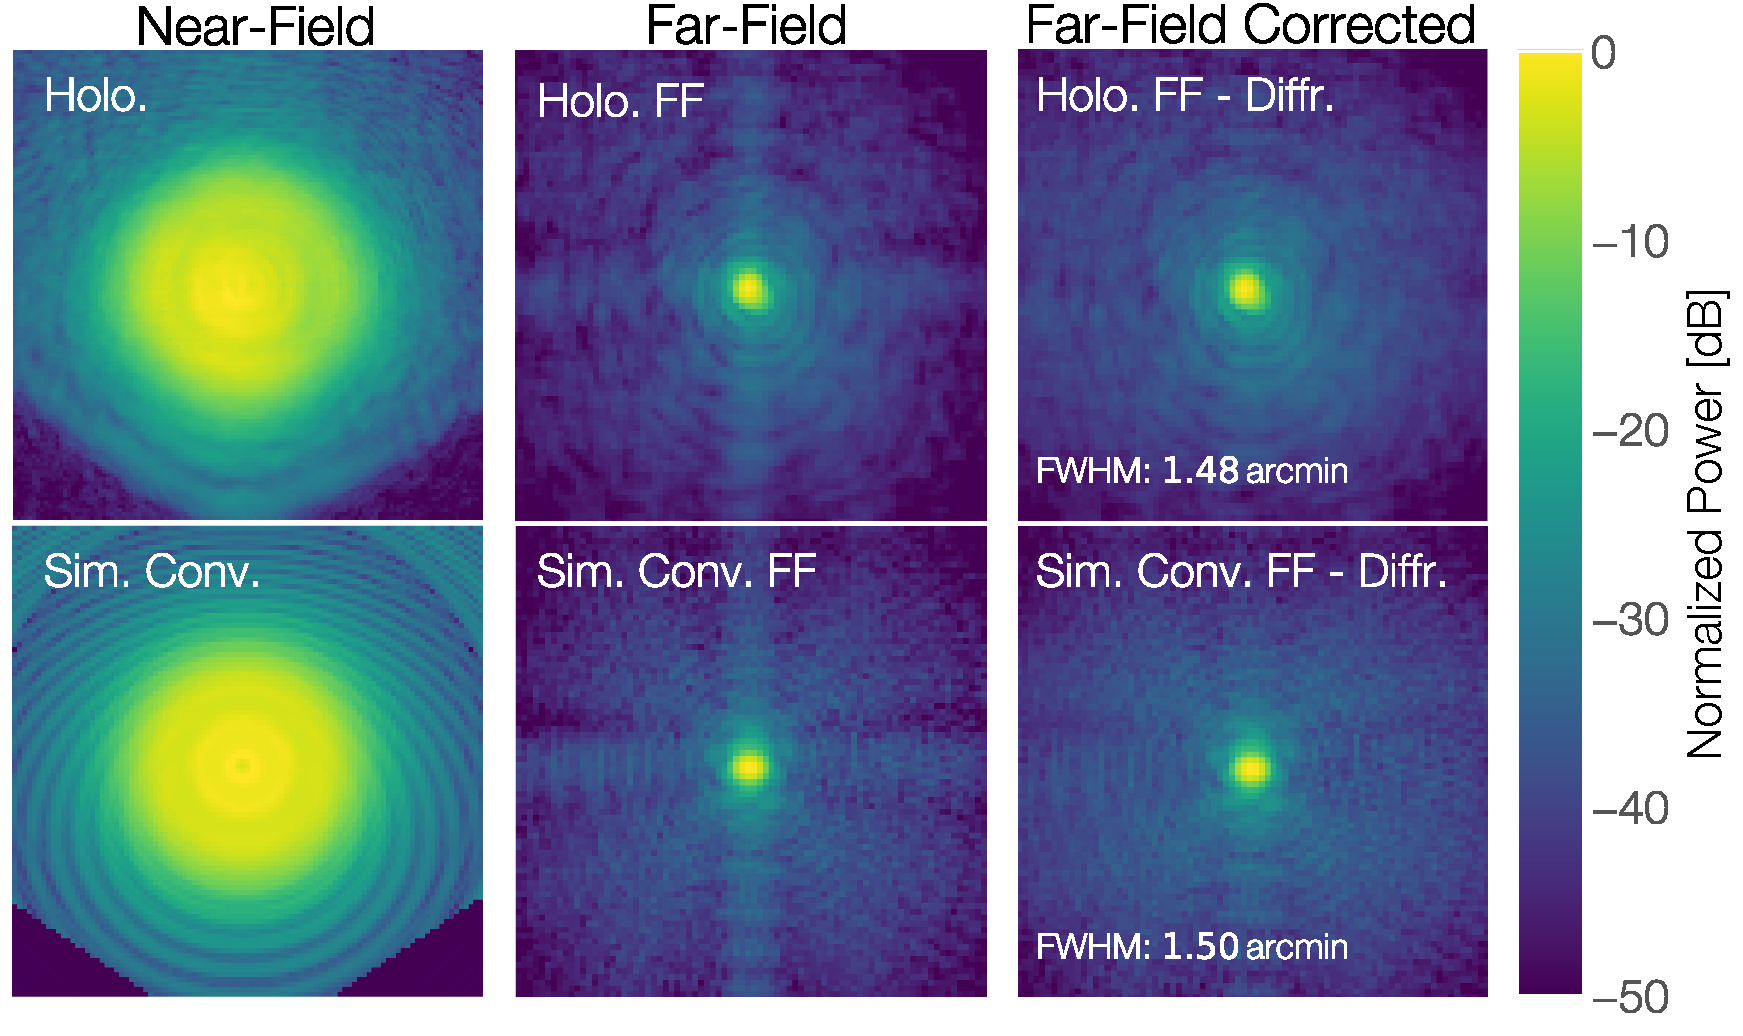
\includegraphics[width = .9\textwidth]{Figures/forward_convolve_highres.pdf}
    \caption{Forward modelling method with the F150 band-averaged holography data. Column 1:  Near-field holography data(top) and convolved simulation with a scattering term(bottom).  Square is $12\times12\,$cm.  Column 2: Far-field holography data(top) and convolved simulation with a scattering term(bottom).  Diffraction spikes consistent with a convolution from a square aperture are present in both the measured far-fields and the simulated far-fields, due to the source horn having a rectangular aperture face.  Square is $20\times20\,$arcmin.  Column 3:  Far-field holography data with diffraction model removal(top) and convolved simulation with a scattering term with diffraction model removal(bottom). Square is $20\times20\,$arcmin.}
    \label{fig:forward_model}
\end{figure*}
\section{Forward Modelling}
\label{sec:forward_model}
\begin{figure*}[t]
    \centering
    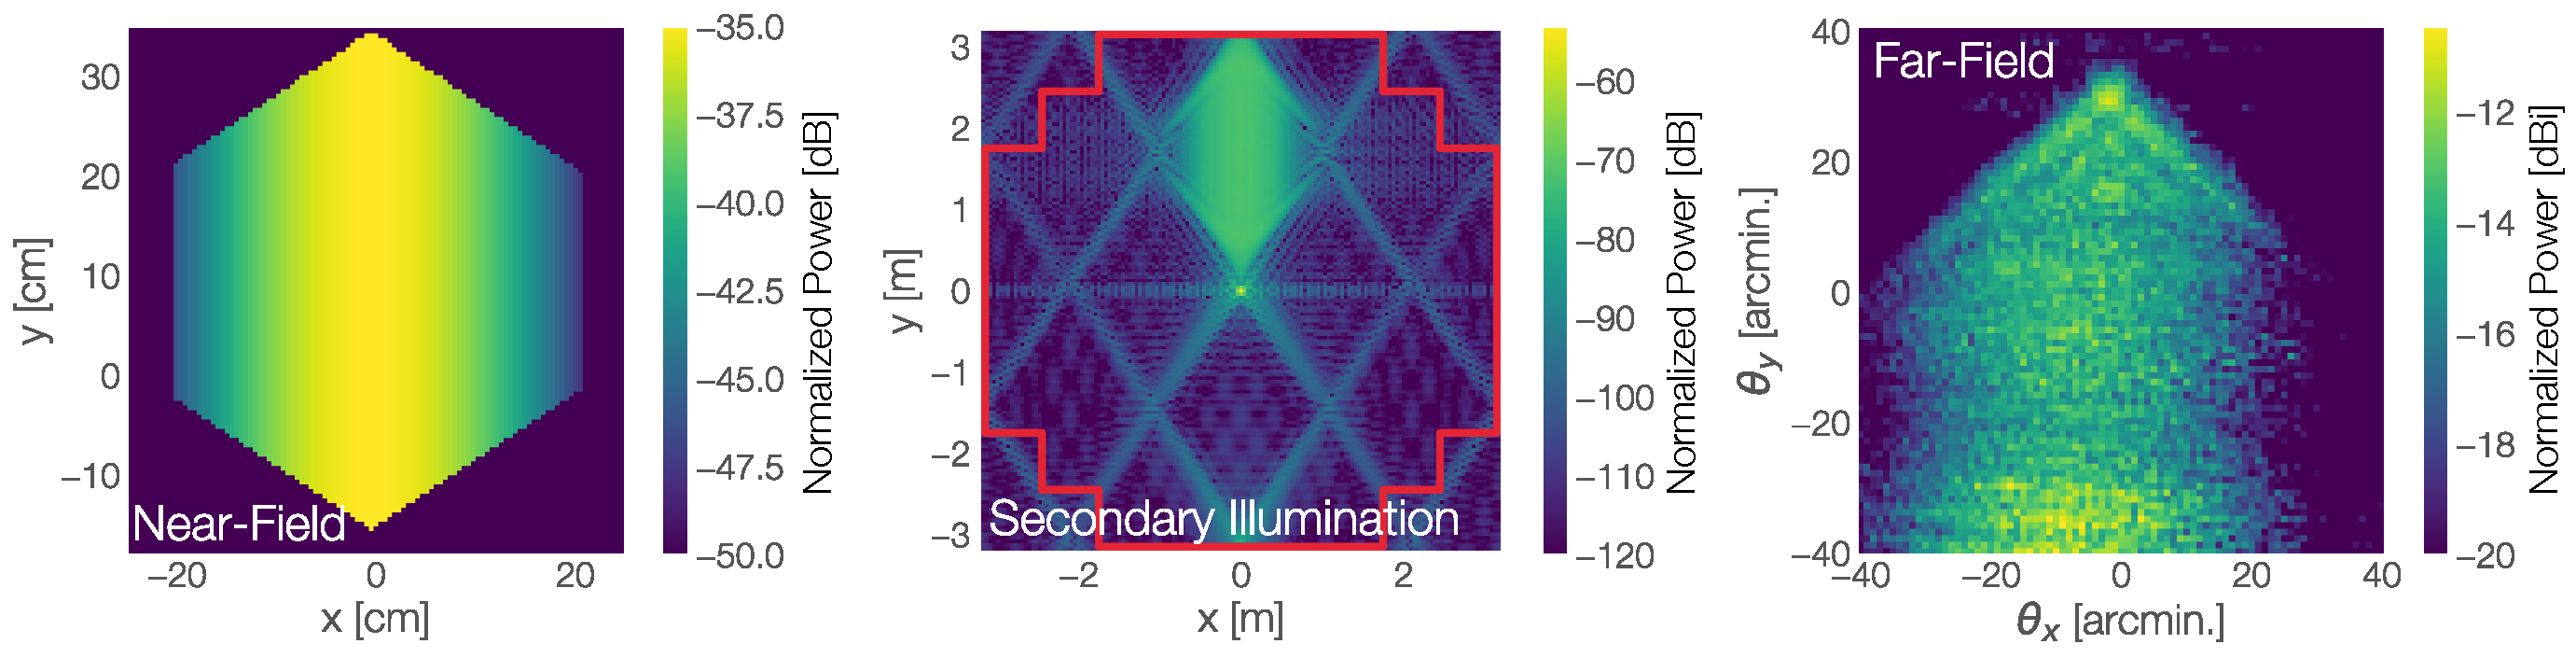
\includegraphics[width = .95\textwidth]{Figures/scatter_model.pdf}
    \caption{Simulated scattering term (power) in the near-field(left), at the secondary illumination(middle) and propagated to the far-field(right).  Each subplot is the band-averaged simulation over all F150 frequencies.}
    \label{fig:scattering_forward}
\end{figure*}
As introduced in Section~\ref{sec:results}.~\ref{sec:prop_fields}, the holography source emits from a rectangular feedhorn, and therefore result in a convolution of the electromagnetic field from the optics tube with the field pattern on the feedhorn aperture.  Convolving the simulated fields increases the F90(150) far-field beam by 12.2(4.7)\% and results in horizontal and vertical diffraction spikes in the raw far-field calculation~\cite{Goodman2005-ne}.

We carry out the forward modelling by building a simulation of the optics tube beam pattern at the measurement plane.  This model includes an empirical model of the scattering of the optics tube with the hexagonal outline to model the boundary of the optics tube window, and a similar amplitude and phase to what is measured.  The resulting simulated F90(150) beam matched the measured FWHP beam width within in 1.73(0.7)\%.  The simulation also had the horizontal and vertical diffraction spikes in the far-field due to the impact of the convolution with the holography source feed pattern~\cite{Goodman2005-ne}.  The full forward modelling process is shown in Figure~\ref{fig:forward_model}.
\begin{table}[ht]
\centering
\begin{tabular}{|c|c|c|c|c|}
\hline
F\,[GHz] & \multicolumn{3}{c|}{S/N [dB]}\\
& NF& Sec.& FF\\
\hline
 90      & 0 & 20.3  & 32.8\\
         & 20& 21.7 & \\
         & 40& 37.0 & \\
         & 60& 45.4 & \\
 150     & 0 & 15.0 & 32.3 \\
         & 20& 18.0 & 39.3\\
         & 40& 35.5 & 43.8\\
         & 60& 46.0 & 43.8\\
 \hline
\end{tabular}
\caption{Near-field measurement signal-to-noise and resulting far- side-lobe power (at the secondary illumination and into the far-field).}
\label{tab:fft_sn}
\end{table}
For visualization purposes, these spikes are removed by subtracting a model $D(\theta_x,\theta_y)$ (amplitude of the electric field) consisting of a $\sinc$ function with a Gaussian width along its narrow direction equal to the beam width (Eq.~\ref{eq:model_conv}), where $\theta_x$ and $\theta_y$ are elevation and azimuth, and we fit the 2 parameters $\sigma_{\theta_x}$ and $\sigma_{\theta_y}$.  This model is based on the predicted Fraunhofer diffraction pattern from a rectangular aperture~\cite{Goodman2005-ne} (e.g., the feed) and was shown to match the simulations.
\begin{equation}
    D(\theta_x,\theta_y) = \exp^{-(\theta_x^2/4\sigma_{\theta_x}^2 +\theta_y^2/4\sigma_{\theta_y}^2 )}\sinc{\theta_x}\sinc{\theta_y}
    \label{eq:model_conv}
\end{equation}
The holography measurements showed scattering from within the optics tube (hexagonal shape at ~-20\,dB in Figure~\ref{fig:beam_measurements_all}).  To understand how this scattering propagates through the telescope, we add a scattering term (with both amplitude and phase) to the simulated beam, and then propagate this beam into the far-field.  We also investigate how the side-lobes measured outside the main beam (Fig.~\ref{fig:beam_measurements_all}) propagate into the far-field (Fig.~\ref{fig:scattering_forward}).  Reflections are known to be a problem in near-field beam mapping~\cite{2020JLTP..199..156Y,7740846,387181}.  However, the inferred amplitude of the probe is small, and we do not correct for reflections.  The side-lobe spreads out and is localized to 2 meters from the center of the primary and secondary mirrors, and then leads to a $0.85^{\circ}$ diffuse structure on the sky that is at the $\approx -15$\,dBi level.
\section{Measurement Requirements}
\label{sec:err_prop}
Here, we discuss the measurement requirements to meet specific far-field resolution from near-field data.  Near-field beams with four signal-to-noise levels are propagated into the far-field (for 90\, and 150\,GHz near-field beams); we simulate the near-fields to have 0, 20, 40, and 60\,dB signal-to-noise.  The signal-to-noise propagated to the secondary illumination and to the far-field is listed in Table~\ref{tab:fft_sn}. 
\begin{table}[htb]
\centering
\begin{tabular}{|c|c|c|c|c|c|c|}
\hline
F\,[GHz] & \multicolumn{2}{c|}{NF [cm]}&\multicolumn{2}{c|}{Sec. [m]} & \multicolumn{2}{c|}{FF [arcmin]} \\
 & Size & Res. & Size & Res.& Size & Res.\\ \hline
 90 & 50& 0.25 & 9.52& 0.13& 119.72 & 0.60\\
 150 & 50& 0.20 &6.66 &0.06 &128.40&0.52\\
 \hline
\end{tabular}
\caption{Near-field scan size and resolution, and resulting scan size and resolution at the secondary illumination and in the far-field.}
\label{tab:fft_grid}
\end{table}
When planning the near-field scan, we consider the resolution and how the near-field grid propagates into the far-field, due to the Fourier relationship between near- and far-fields (Eq.~\ref{eq:fft}).  Table~\ref{tab:fft_grid} summarizes the scan size and resolutions and resulting far-field size and resolution grids used in the holography measurements.
